\section{Proposed Approach}
\label{sec:approach}

In this section, we introduce our approach to support bottom-up language product lines. Our approach is explained in two parts. First, we present some meta-language facilities needed to define a language product line in terms of language modules, features, and variability models. Then, we introduce a reverse engineering algorithm to automatically build a language product line from a set of existing DSL variants that have been built through the clone-and-own approach. 

\subsection{Meta-language Facilities to Language Product Lines}
\label{sec:meta-langauges}

As we explained earlier, the definition of a language product line requires support for languages modularization and variability management. This support should be materialized in some facilities at the level of the meta-languages used during the language development process. In the following, we explain how we use and extend current meta-languages to this end. 

\subsubsection{Support for Language Modularization}

%During the construction of a language product line, language designers should implement DSLs in the form of interdependent \textit{language modules} which materialize language features. Each language module, provides a set of language constructs, and a DSL is obtained from the composition of two or more language modules. 

Just as in typical software modularization \cite{Tripakis:2003}, languages modularization supposes the existence of two properties: separability and composability. \textit{Separability} refers to the capability of designing and verifying language modules independently of other language modules it may require. Separability relies on the definition of interfaces specifying the interactions between language modules. In turn, \textit{composability} refers to the capability of integrate several language modules to produce a complete and functional DSL. Composability relies on the usage of the interfaces between language modules in such a way that they can interchange both control and information.

\vspace{2mm}
\textbf{\textit{Language interfaces to achieve separability.}} We propose the use of language interfaces to achieve separability of language modules. In particular, we propose the classical required and provided interfaces explained below. 

\vspace{2mm}
\textit{Required interfaces.} The purpose of a required interface is to support independent development of language modules. In that sense, a required interface is a mechanism that allows language designers to declare the needs that a language module has towards other modules while assuming that their needs will be eventually fulfilled. Suppose for example the development of a language module for finite state machines. This language module needs some additional abstractions such as constraints to express guards in the transitions. Using a required interface, language designers can declare those needs as a set of required constructs (e.g., \textsl{Constraint}) and focus on the definition of the constructs which are proper to finite state machines (e.g., \textsl{State}, \textsl{Transition}, \textsl{Triggers}). 

As the reader might infer from the last paragraph, the needs of a language module can be materialized in the form of required constructs. In assuming so, the specification of a language module would be composed of a set of actual constructs, which are being implemented by the module; and a set of required constructs, which represent needs to other modules. This approach would result useful to support the modularization scenario called aggregation where the needs of language modules are entire constructs implemented in foreign modules. However, a finer level of granularity might be necessary to support other modularization scenarios such as extension where the needs are not necessarily entire constructs but finer elements such as properties or operations. 

Based on this reasoning, we propose a mechanism to enable the capability to distinguish whether a given language specification element (i.e., meta-class, property, operation, parameter, enumeration, etc) corresponds to an actual implementation or a required declaration. The proposed mechanism is an extension to the EMOF meta-language that introduces the notion of \textit{virtualization}. Using this extension, language designers can define virtual specification elements expressing needs of the module. Non-virtual specification elements are actual implementations of the language module. The required interface of a language module is the set of virtual elements it contains within its specification.

Fig. \ref{fig:fig-req-example-fig} illustrates the use of required interfaces through the example introduced before regarding a language module for finite state machines that requires a constraint language. In that example, the constructs proper the state machines are non-virtual elements since they correspond to actual implementation of such abstractions. In turn, the constraints to express the guards in the transitions are expressed as a virtual construct called \textsl{Constraint} that provides a virtual operation action called \textsl{eval()} which is used in the specification of the semantics of the meta-class \textsl{Transition}. 

\begin{figure}
  \centering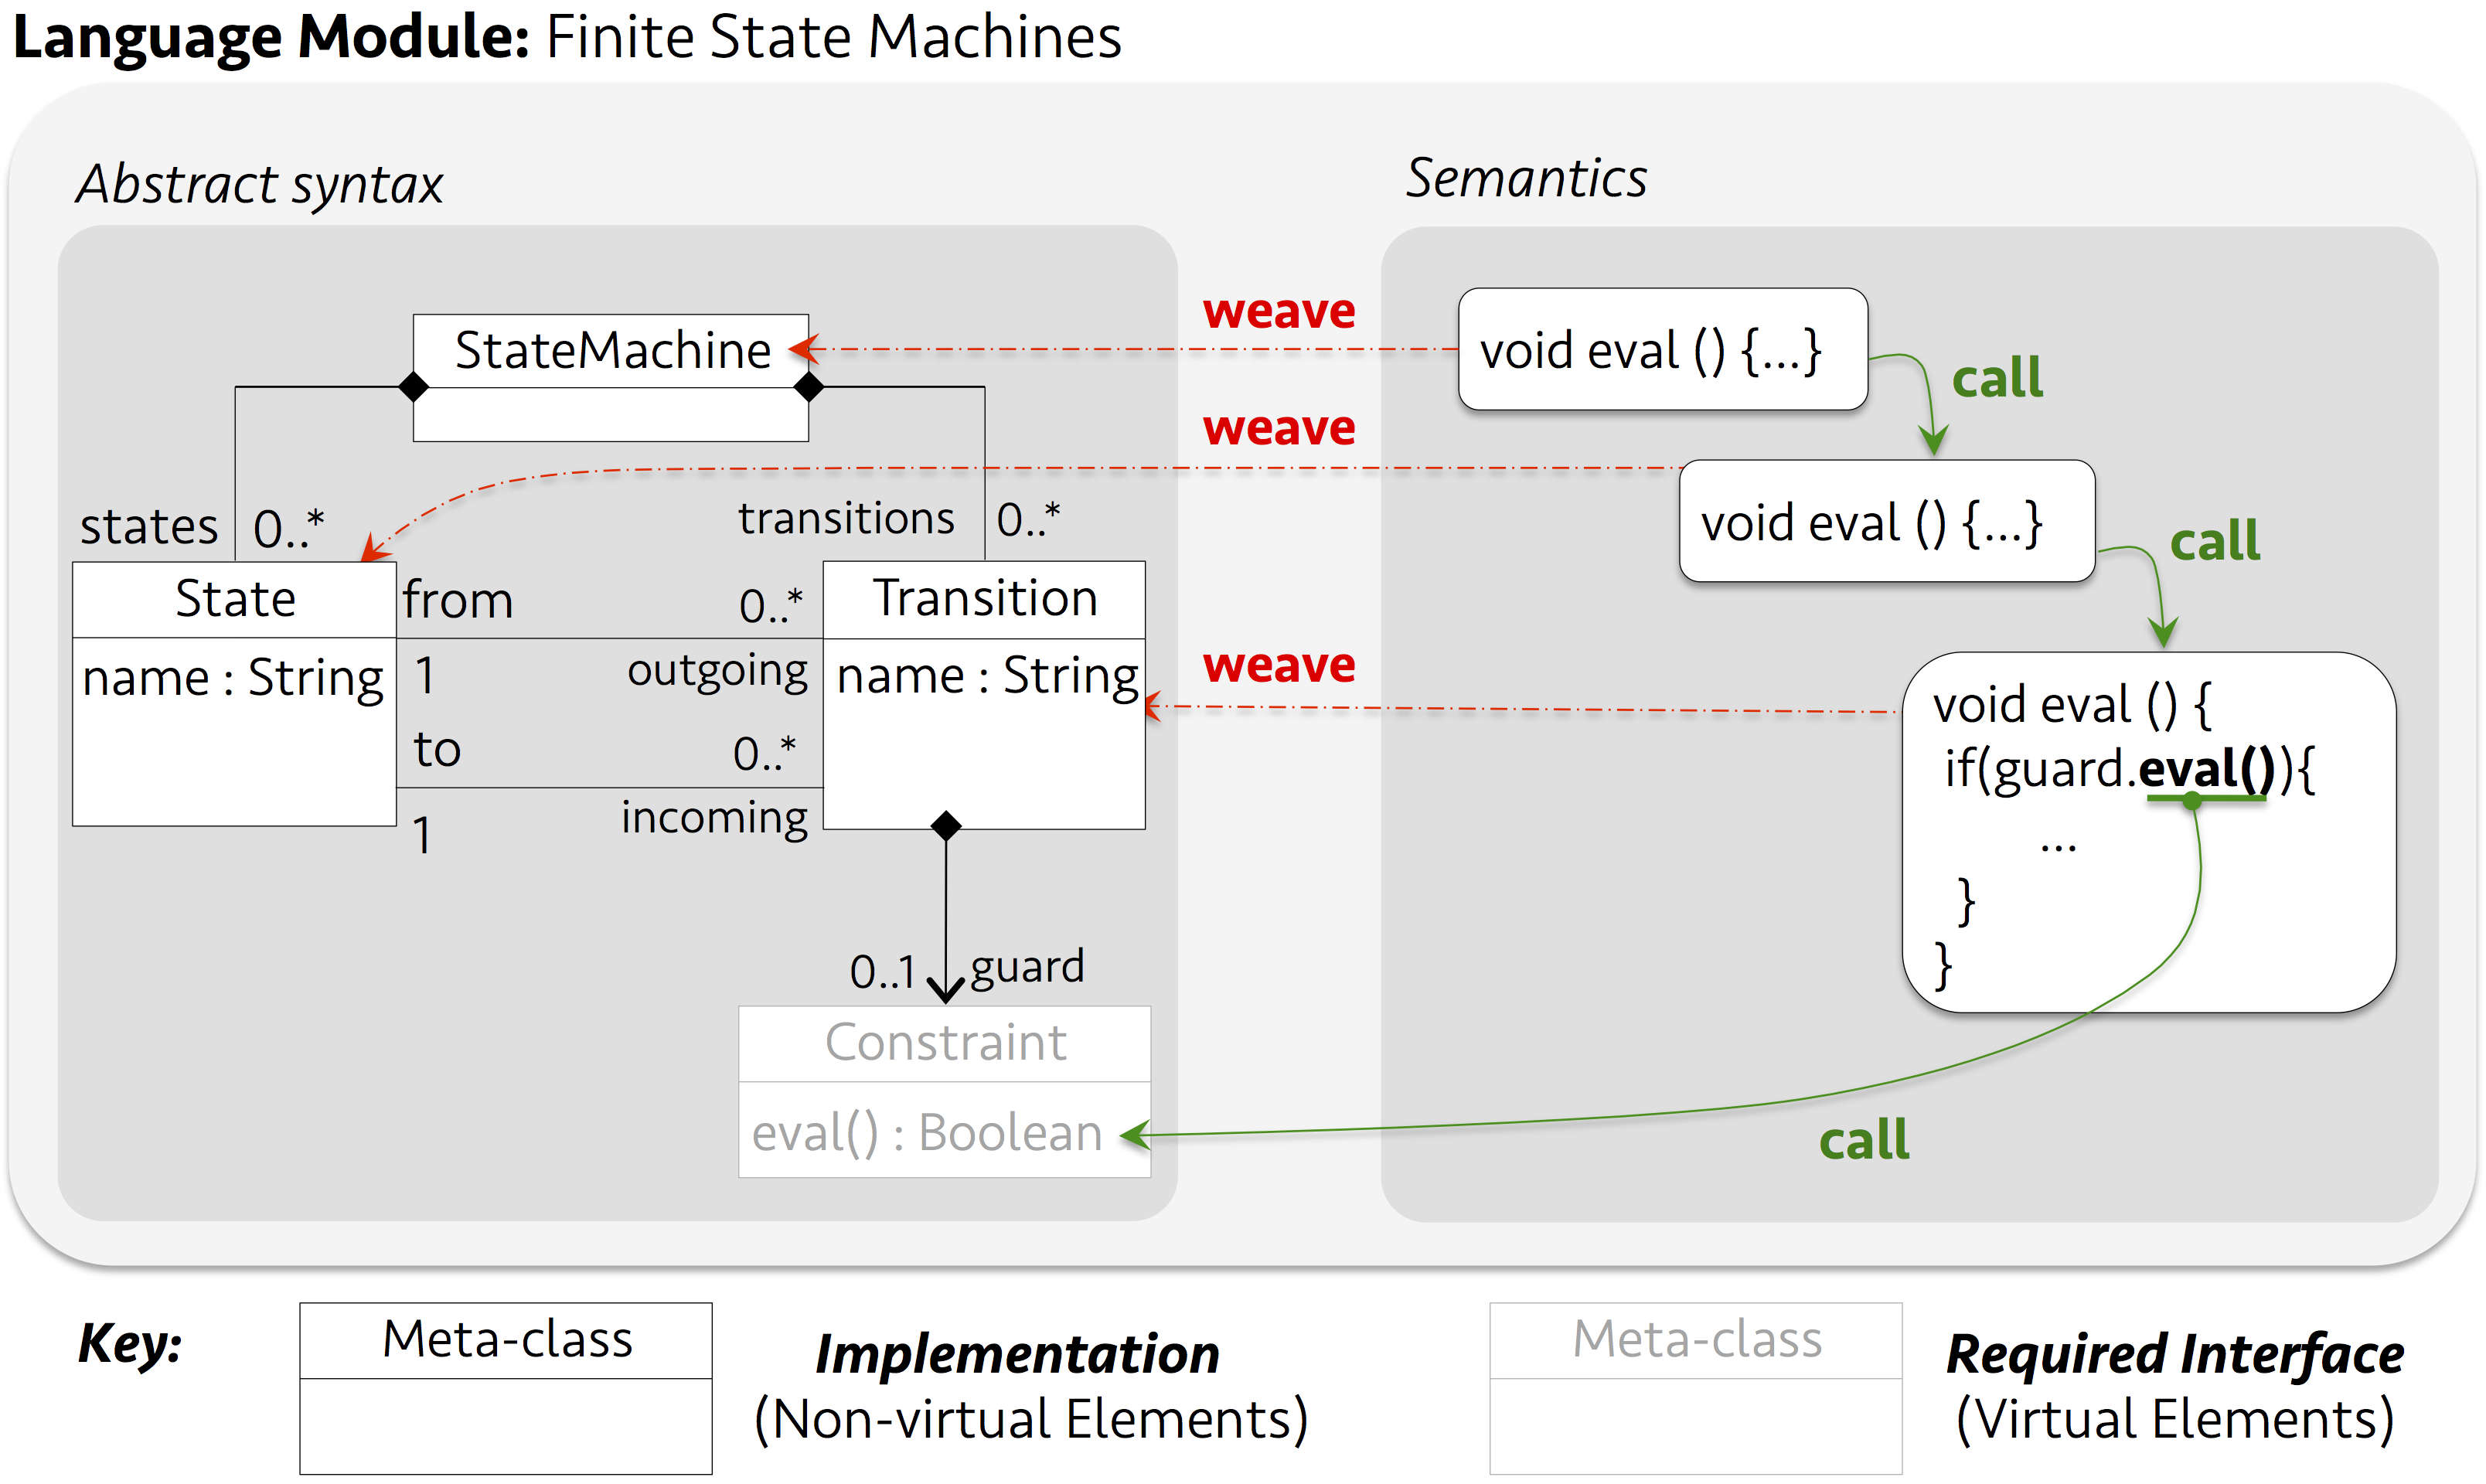
\includegraphics[width=0.86\linewidth]{images/fig-req-example-fig.png}
  \caption{Example of the use of required interfaces}
  \label{fig:fig-req-example-fig}
\end{figure}

\vspace{2mm}
\textit{Provided interfaces.} In our approach, the purpose of provided interfaces is to enable information hiding in the modular development of DSLs. That is, to distinguish between the information that specifies the functionality offered by the language module from the information corresponding to the implementation details behind such functionality. Consider for example a language module that offers the capability to express and evaluate constraints. Using a providing interface, language designers can express the essential functionality of the module i.e., expression and evaluation of constraints; and hide the implementation details and auxiliary concepts needed to achieve such functionality e.g., context management.

To support the definition of provided interfaces, we propose to extend EMOF with the notion of \textit{module visibility}. This extension allows to classify a certain specification element as either \textsl{\textbf{public}} or \textsl{\textbf{private}} according to its nature. For example, a language designer can classify a meta-class as \textsl{\textbf{public}} meaning that it represents essential functionality of the module so can be used by external modules and it belongs to the provided interface. Naturally, if the meta-class is classified as \textsl{\textbf{private}} it cannot be used by external modules and it cannot be considered as part of the provided interface. Note that the notion of module visibility is different from the notion of visibility already defined in EMOF. The later is associated to  certain access constraints of model elements with respect to the package in which they are implemented.

Fig. \ref{fig:fig-prov-example-fig} illustrates the use of provided interfaces through the example regarding the constraints module. Since the main functionality of the module is to define and evaluate constraints, the meta-classes included in the provided interface (so those one defined as \textsl{\textbf{public}} in terms of module visibility) are: \textsl{ConstrainedProgram} and \textsl{Constraint} including the operations that implement their semantics.

\begin{figure}
  \centering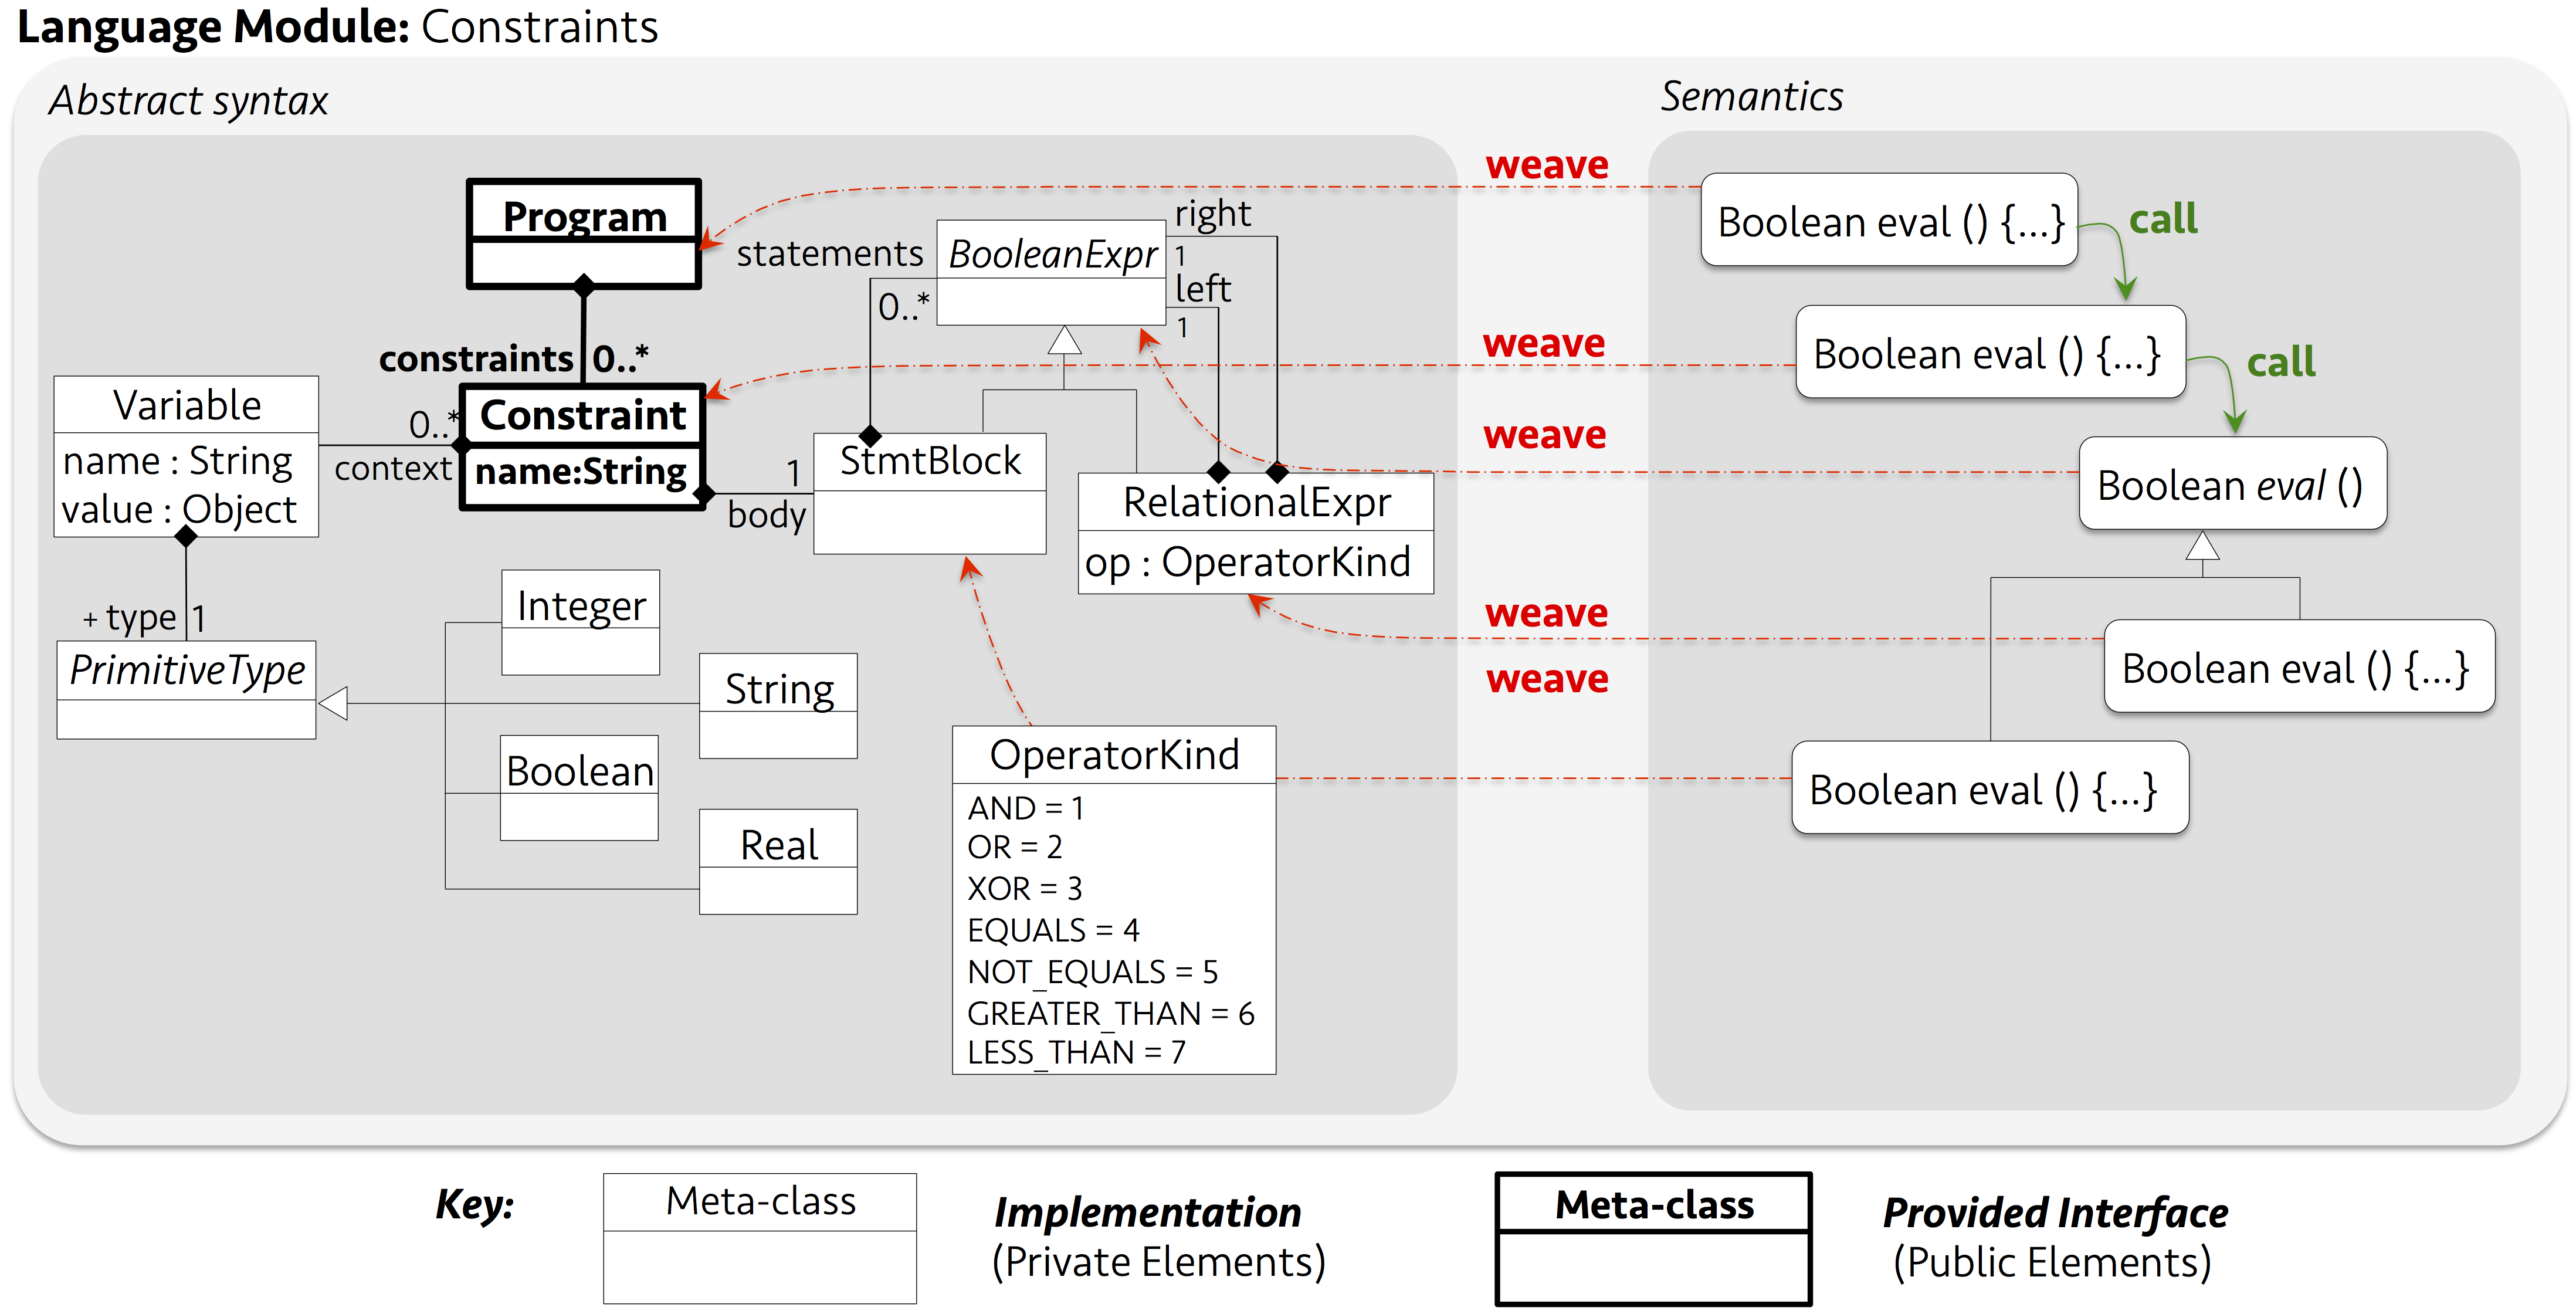
\includegraphics[width=1\linewidth]{images/fig-prov-example-fig.png}
  \caption{Example of the use of provided interfaces}
  \label{fig:fig-prov-example-fig}
\end{figure}

\vspace{2mm}
\textbf{\textit{Interfaces binding to achieve composability.}} Now, we need to define the way in which those interfaces interact each other at the moment of the composition. In doing so, it is important to conciliate two different (and potentially conflicting) issues. Firstly, safe composition of the involved language modules should be guaranteed; we need to check the compatibility between a providing and a requiring language module by verifying that the functionality offered by the former actually fulfills the needs of later. Secondly, there must be some place for substitutability; compatibility checking should offer certain flexibility that permits to perform composition despite some differences in their definitions. This is important because when language modules are development independently of each other, their interfaces and implementations not always match \cite{Gschwind:2012}.

To deal with the aforementioned issues, we propose an approach for compatibility checking. It is at the same time strict enough to guarantee safe composition, and flexible enough to permit substitutability under certain conditions. Concretely, we propose to extract both required and provided interfaces in the form of \textit{model types} \cite{Steel:2007}. The model type corresponding to the required interface contains the virtual specification elements of a language module whereas the model type corresponding to the provided interface the model type contains its public specification elements. The relationship between a model type and a language module is called \textsl{\textbf{implements}} and it is introduced by Degueule et al. \cite{Degueule:2015a}. 

In order to perform compatibility checking, we use the sub-typing relationship --introduced by Guy et al. \cite{Guy:2012}-- between the model types corresponding to the provided and the required interfaces. This relationship imposes certain constraints that guarantee safe composition while permitting some freedom degrees thus introducing some flexibility. In particular, under this definition of sub-typing the most obvious manner to guarantee safe composition is to check two conditions: (1) all the needs expressed in the requiring model type are furnished in the providing model type (\textbf{total} sub-typing); and (2) the two model types have exactly the same shape (\textbf{isomorphic} sub-typing). However, this definition of sub-typing also provides two dimensions of flexibility: \textbf{partial} sub-typing and \textbf{non-isomorphic} sub-typing. 

The main principle behind partial sub-typing is that not all the needs expressed in the required model type must be provided by the provided one. In that case, compatibility checking corresponds to verify that the sub-set of elements that match in the model types are compatible. Then, the result of the composition is a third language module with a resulting required interface that contains those needs that have not been satisfied by the providing language module. 

As an example suppose a language module for finite state machines that needs not only constraints for expressing guards in the transitions, but also action scripting constructs to express the behavior of the states. In such a case, a constraint module will fulfill the first need but not the second one. Thanks to partial sub-typing, we can perform compatibility checking only on the constructs associated to the constraints and, if they are compatible, then compose those language modules. The result will be a language module having the constructs for state machines and constraints but that still needs action scripting constructs defined in its required interface.

The principle behind isomorphic sub-typing is that the needs in the requiring interface are not always expressed exactly as the functionality offered by the providing module is expressed in the providing interface. For example, model type in Fig. \ref{fig:fig-req-example-fig} expresses the needs in terms of constraints of state machines through a class \textsl{Constraint} with an operation \textsl{eval()}. If we want to use OCL to satisfy these needs, then we will find that there is not a class constraint but \textsl{OclExpr}. Besides, the operational semantics might be implemented differently. In this case, we need an adapter that permit to find the correspondences among the elements of the model types. 

At the implementation level, in the current state of our approach we support partial sub-typing and some particular cases of non-isomorphic sub-typing. We still need some research to fully support non-isomorphic sub-typing in a general specially at the moment of the composition. 

\vspace{2mm}
\textit{Language modules composition.} Once the compatibility between two language modules is correctly checked, the next step is to compose the language modules to integrate their functionality i.e., the needs of the requiring module are fulfilled with the services offered by the provided one.  In our approach, this composition is performed in two phases. First, there is a matching process that identifies one-to-one matches between virtual and public elements from the required and provided interface respectively. This match can be identified automatically by comparing names and types of the elements (where applicable). However, the match can be also specified manually in the case of non-isomorphism.

Once the match is correctly established, the composition process continues with a merging algorithm that replaces virtual elements with public ones. When the process is finished, we re-calculate both provided and required interfaces. The provided interface of the composition is re-calculated as the sum of the public elements of the two modules under composition. In turn, the required interface of the composition is re-calculated as the difference of the required interface of the required module minus the provided interface of the providing module. 

\subsubsection{Support for Language Variability Management}

The challenge towards supporting the variability existing in a language product line is that such variability is multi dimensional. Because the specification of a DSL involves several implementation concerns\footnote{Just as traditional general purpose languages, domain specific languages are typically defined through three implementation concerns: abstract syntax, concrete syntax, and semantics \cite{Harel:2004b}.}, then there are several dimensions of variability i.e., abstract syntax variability, concrete syntax variability, and semantic variability \cite{Cengarle:2009,Gronniger:2011}. Abstract syntax variability refers to the capability of selecting the desired language constructs for a particular type of user. In many cases, constructs are grouped in \textit{language features} to facilitate the selection. Such grouping is motivated by the fact that selecting constructs can be difficult because a DSL usually has many constructs, so a coarser level of granularity is required. In turn, concrete syntax variability refers to the capability of supporting different representations for the same language construct. Finally, semantic variability refers to the capability of supporting different interpretations for the same language construct.

In this section we present a strategy to deal with this type of variability. To this end, we present an approach to represent the variability existing in a language product line. Then, we explain how we can use the variability models to configure concrete DSLs. As the same as our approach to language modularization, our approach to variability management is scoped to abstract syntax and semantics; concrete syntax --and hence, concrete syntax variability-- is not being considered in the solution. 

\vspace{2mm}
\textbf{\textit{Modeling multi-dimensional variability.}} A solution to represent abstract syntax variability and semantic variability should consider two main issues. Firstly, the definition of the semantics has a strong dependency to the definition of the abstract syntax --the domain-specific actions that implement the semantics of a DSL are weaved in the meta-classes defined in the abstract syntax--. Hence, these dimensions of variability are not isolated each other. Rather, the decisions made in the configuration of the abstract syntax variability impact the decisions that can be made in the configuration of the semantic variability. For example, there is a variation point for the case of state machines that proposes different ways to deal with conflicting transitions. However, conflicting transitions are only possible within hierarchical state machines. Hence, if the state machine DSL does not support hierarchical states, then it makes no sense to configure this semantic variation point. 

The second issue to consider at the moment of dealing with language variability management is that a semantic variation point might be transversal to several meta-classes. For example, there is a semantic variation point in hierarchical state machines that corresponds to decide if the state machine follows either the run-to-completion policy or if it supports simultaneous events \cite{Crane:2007}. In any case, the implementation of this semantics involves code in domain-specific actions for the \textsl{StateMachine} and \textsl{Region} meta-classes. Moreover, if the involve meta-classes are introduced by different language modules in the abstract syntax, then the semantic variation point depends of two features. Hence, the relationship between a feature in the abstract syntax and a semantic variation point is not necessarily one-to-one. 

Currently, we can find several approaches to support multi dimensional variability (e.g., \cite{Rosenmuller:2011}). Some of those approaches have been applied concretely to language product lines. In particular, they propose to model all the dimensions of variability through feature models and then to establish dependencies among them. However, the differ in the way in which the features are organized. For example, in some cases there is a unique variability model with one branch for each dimension of variability whereas there are other approaches that propose the use of one feature model for each dimension and then they use cross-tree constraints to represent the dependencies among the dimensions. 

In this article we propose a different approach to deal with language variability management. Concretely, we propose to combine the use of feature models with orthogonal variability models; feature models are used to model abstract syntax variability and orthogonal variability models are used to model semantic variability. Fig. \ref{fig:languages-variability-modeling} shows illustrates our approach. At the top of the figure, we find a feature model which each feature represents one language module. At the bottom, we have an orthogonal variability model that represents the semantic variation points existing among those language modules. As the reader might imagine, each of the variants of the variation points are associated not only to a particular module but also to the corresponding domain-specific actions associated to its implementation. 

\begin{figure}
  \centering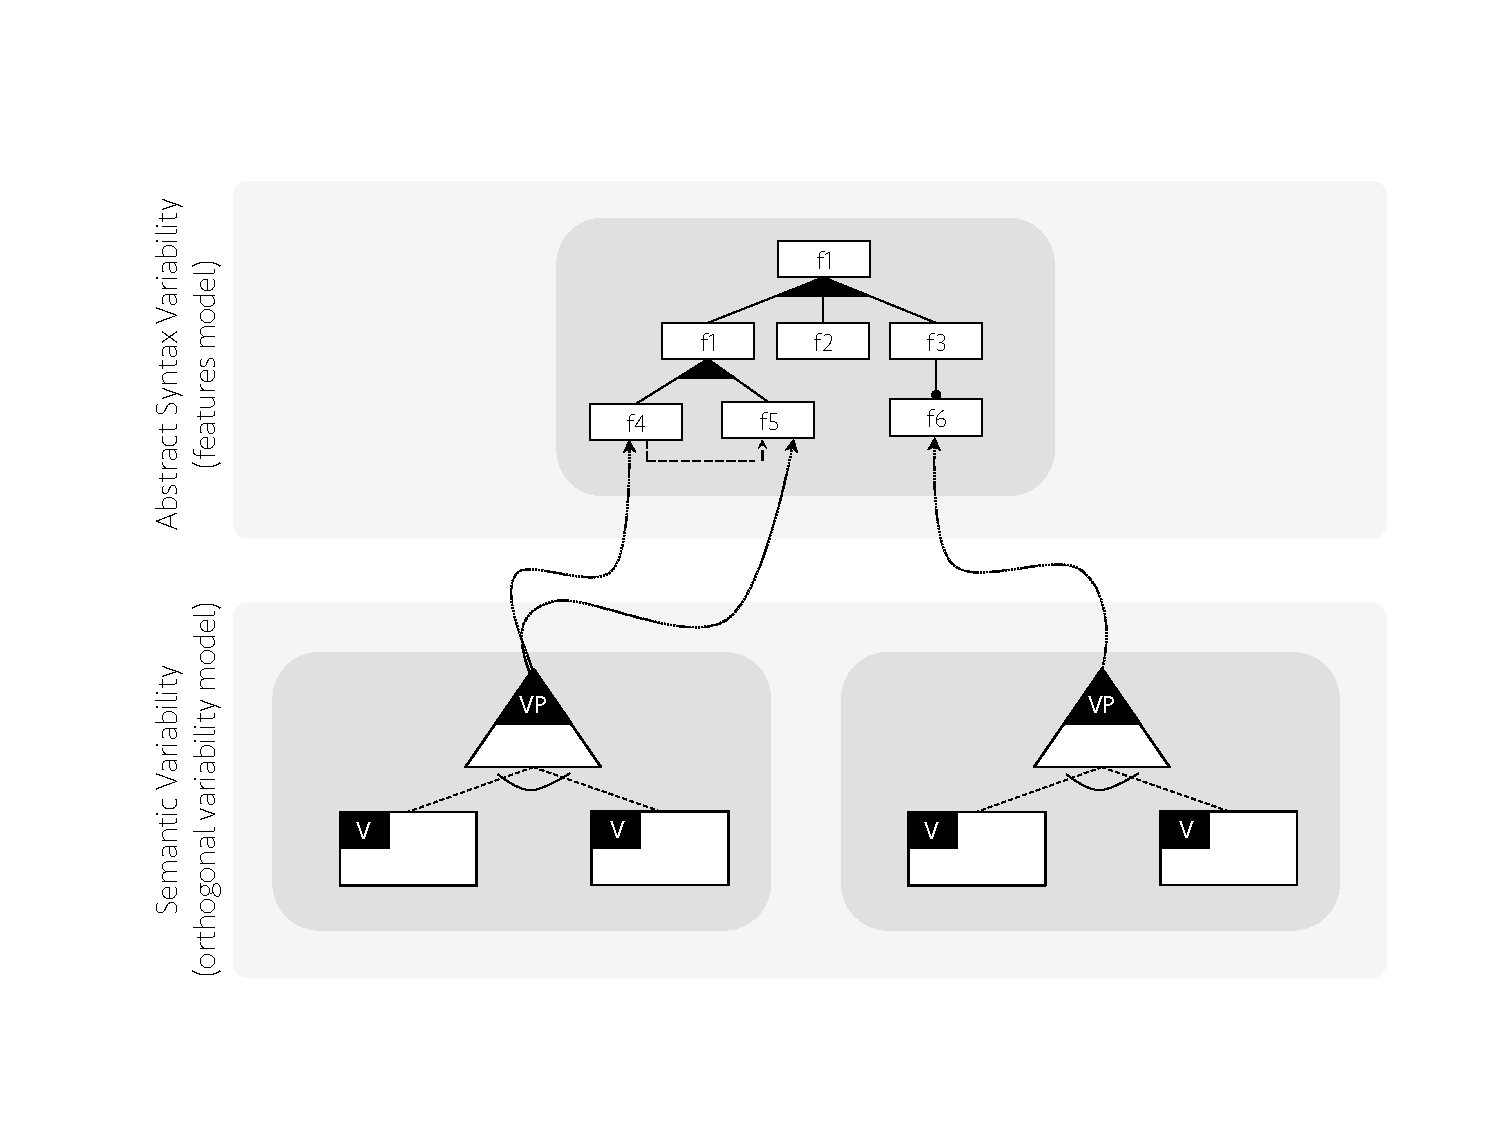
\includegraphics[width=0.84\linewidth]{images/languages-variability-modeling-fig}
  \caption{Approach to represent multi-dimensional variability in language product lines}
  \label{fig:languages-variability-modeling}
\end{figure}

\vspace{2mm}
\textit{Why orthogonal variability models?} An inevitable question that we need to answer at this point is: why we use orthogonal variability models instead of using feature models as proposed by current approaches? The answer to this questions is three-fold:

\vspace{2mm}
\textit{(1) The structure of orthogonal variability models is more appropriated.} As explained by Roos-Frantz et al. \cite{Roos-Frantz:2012}, feature models and orthogonal variability models are similar. However, they have some structural differences. One of those differences is that whereas a feature model is a tree that can have many levels, an orthogonal variability model Is set of trees each of which has two levels. Each tree represent one variability point and its children represent variants to that variation point. 

Semantic variation points are decisions with respect to a particular segment of the semantics of a language. Although those decisions can have some dependencies among them --a decision \textit{A} might force a decision \textit{B}-- they can hardly be organized in a hierarchy. Indeed, we conducted an experiment where we use feature models to represent semantic variation points, and we always obtained two-level trees: the first level corresponds to the name of the variation point and its children represent the possible decisions. This fact suggests that orthogonal variability models are more appropriated than feature models to represent semantic variability.  

\vspace{2mm}
\textit{(2) The meaning of orthogonal variability models is more appropriated.} According to \cite{Liebig:2013}, a language feature is a characteristic provided by the language which is visible to the final user. This definition can be associated abstract syntax variability and the use of feature models can be appropriated to represented it. All the approaches on language product line engineering use feature models to this end showing that it is possible and appropriated. 

The case of the semantic variability is different, however. A semantic decision is not a characteristic of a language that we can select or discard. The semantic of a DSL should be always specified if the DSLs is intended to be executable. Rather, a semantic decision is more a variation point that can have different interpretations captured as variants. Note vocabulary fits better in the definitions provided by orthogonal variability models. More than features, we have variation points and variants, which also suggest that the use orthogonal variability models is more appropriate to represent semantic variability.

\vspace{2mm}
\textit{\textbf{Multi-staged DSLs configuration.}} Once the variability of the language product line is correctly specified, and as long as the language features are correctly mapped to language modules, language designers are able to configure and derive DSLs. There are two issues to consider. First, the multi-dimensional nature of the variability in language product lines, supposes the existence of a configuration process supporting dependencies between the decisions of different dimensions of variability. For example, decisions in the abstract syntax variability may impact decisions in semantic variability. Second, language product lines often require multi-staged languages configuration. That is, the possibility of configuring a language in several stages and by different stakeholders.

Multi-staged configuration was introduced by Czarnecki et al. \cite{Czarnecki:2004} for the general case of software product lines, and discussed by Dinkelaker et al. \cite{Dinkelaker:2010} for the particular case of DSLs. The main motivation to support such functionality is to transfer certain configuration decisions to the final user so he/she can adapt the language to exactly fits his/her needs \cite{Dinkelaker:2010}. In that case, the configuration process is as follows: the language designer provides an initial configuration. Then, the configuration is continued by the final user that can use the DSL as long as the configuration is complete. In doing so, it is important to decide what decisions correspond to each stakeholder.

Suppose the scenario introduced in Fig. \ref{fig:languages-configuration-modeling} where the language designer is responsible to configure the abstract syntax variability whereas the language user is responsible to configure the semantics. When the language designer finishes its configuration process, the orthogonal variability models will be available so the final user can perform the configuration of the semantics. This orthogonal variability model will only include the variation points that are relevant to the features included in the configuration of the abstract syntax. Moreover, because each of the semantic variation points are represented separately in a different tree, then we can imagine a scenario where the language designer is able to configure not only the abstract syntax but also some semantic variation points, and then delegate to the final user only the decisions that he/she can take according to its knowledge. 

\begin{figure}
  \centering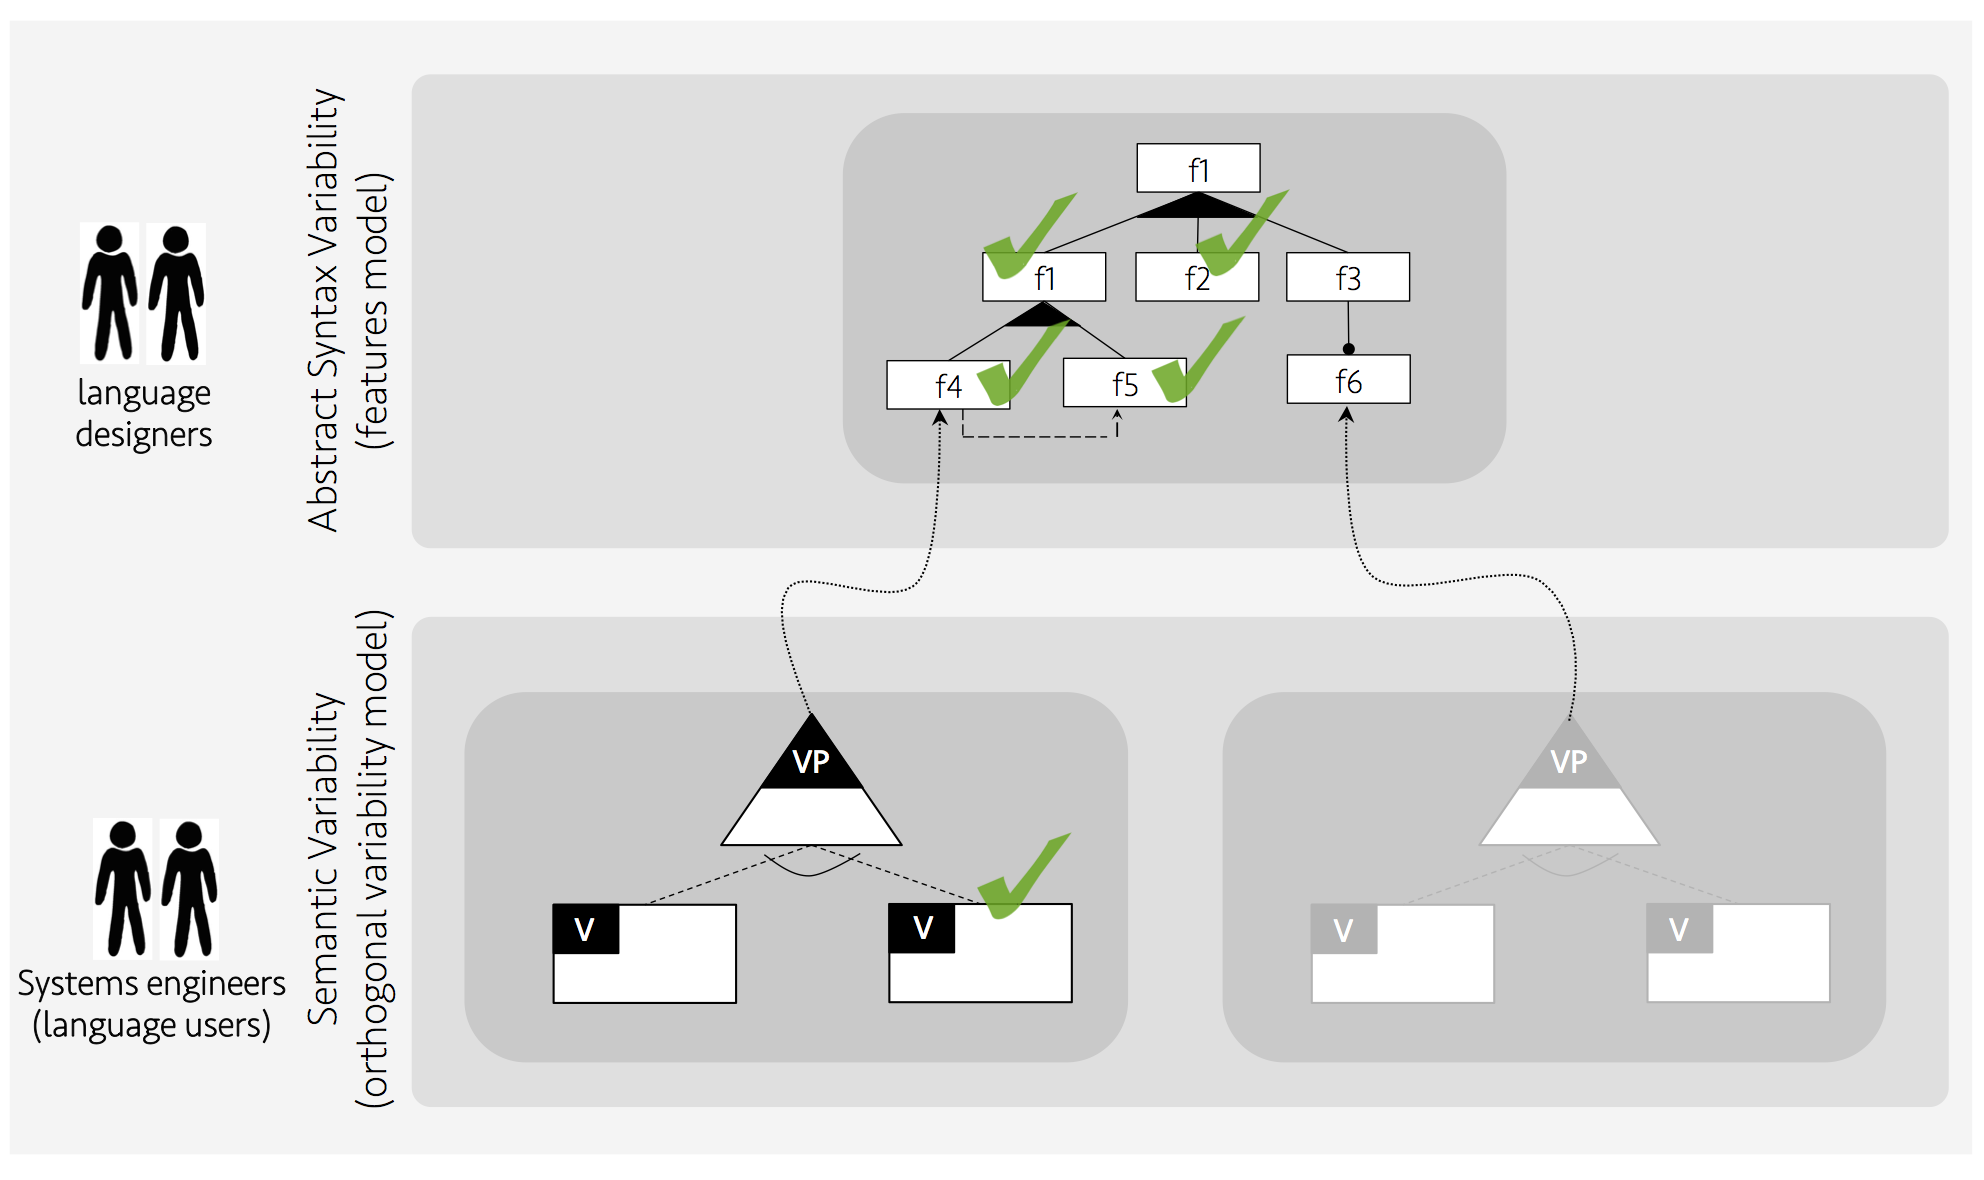
\includegraphics[width=1\linewidth]{images/languages-configuration-fig.png}
  \caption{Approach to support multi-staged configuration of language product lines}
  \label{fig:languages-configuration-modeling}
\end{figure}

\subsection{The Reverse Engineering Process}
\label{sec:reverse-engineering}

In this section, we introduce a reverse engineering strategy for bottom up language product line engineering. Fig. \ref{fig:reverse-engineering} presents an overview of the approach. It receives as input a set of DSL variants implemented according to the development process described in Section \ref{sec:thedevelopmentscenario} and under the technological space introduced in Section \ref{sec:technologicalscope}.

The first step of the process is the extraction of the language modules that implement the features included in the language product line. The process continues with the synthesis of a variability model that captures both abstract syntax and semantic variability. Such a model can be later used to configure and derive concrete DSLs.

\begin{figure*}
\centering
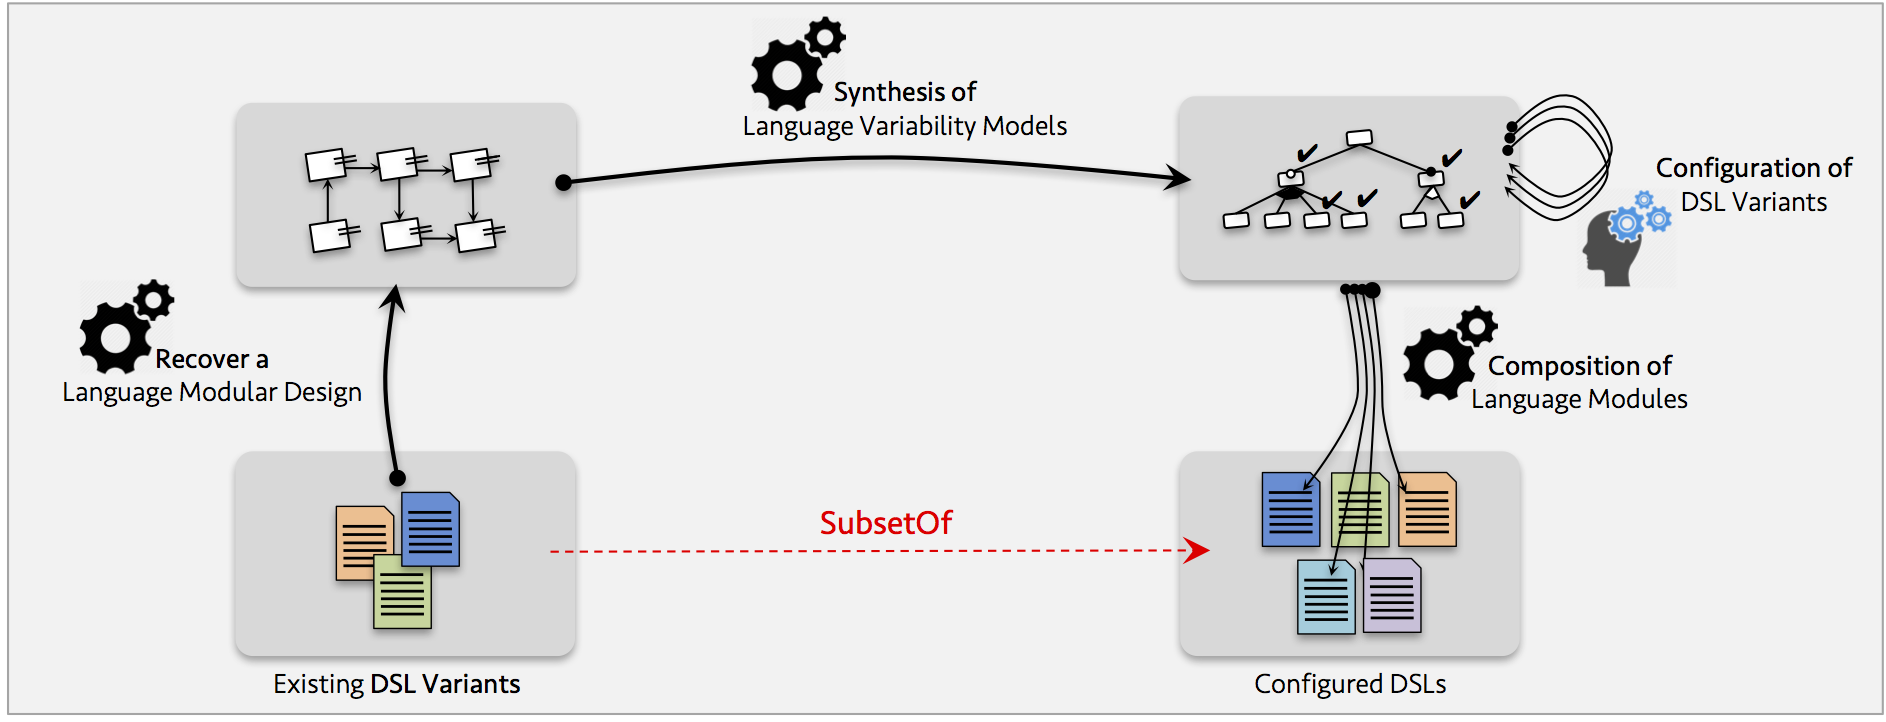
\includegraphics[width=0.95\linewidth]{images/reverse-engineering-overview.png}
\caption{Reverse engineering language product lines: approach overview}
\label{fig:reverse-engineering}
\end{figure*}

\subsubsection{Reverse Engineering Reusable Language Modules}
\label{sec:reverseengineeringmodules}

Let us start the description of our reverse engineering strategy by explaining the way in which we extract the language modules. Roughly speaking, our approach takes the DSL variants given in the input and break them down into several language modules. The purpose of such a breaking down process is to remove all the specification clones existing among the given variants, thus reducing maintenance costs\footnote{Note that we assume the existence such as clones; after all, the involved DSLs were built up by using the clone-and-own approach.}. To this end, we analyze the given DSL variants to detect the existing specification clones. Then, we extract those clones in separate language modules %Our extraction strategy is based on five reverse engineering principles that explained below. %For example, if two DSLs have the constructs A and B, and those constructs are \textit{equal} in terms of their abstract syntax and semantics, then we can extract them and encapsulated them in a separate language module that the involved DSLs might import. 

%Note that this strategy relies on some comparison operators that allow to detect specification clones. These operators might take into consideration not only the abstract syntax, but also the semantics of the language constructs. Then, we need a mechanism to extract the detected specification clones and encapsulate them in such a way that they can be re-composed later with the other parts of the involved DSLs. 

%The first step of our strategy towards bottom up language product lines corresponds to reverse engineering reusable language modules from a given set of legacy DSLs. To this end, we define some comparison operators that allow the identification of replicated language constructs. These operators take into account not only the names of the constructs but also the inter constructs relationships and the semantics. Then, we extract replicated constructs as interdependent language modules whose dependencies are expressed through well defined interfaces. Those language modules can be later assembled among them to build up new DSLs. 

\vspace{2mm}
\textit{\textbf{Principles for language modules' reverse engineering.}} Our strategy for reverse engineering reverse engineering reusable language modules is based on five principles that will be introduced in this section. Then, we explain how we use those principles to extract a catalog of reusable language modules that implement the language features provided by the language product line.

\vspace{2mm}
\textit{\textbf{Principle 1:} DSL specifications are comparable. Hence, specification clones can be detected automatically.} Two DSL specifications can be compared each other. This comparison can be either coarse grained indicating if the two specifications are equal regarding both syntax and semantics, or fine-grained detecting segments of the specifications that match. The latter approach permits to identify specification clones between two DSLs and supposes the comparison of each specification element.

For the technological space discussed in this paper, specification elements for the abstract syntax are metaclasses whereas specification elements for the semantics are domain specific actions. 

\vspace{2mm}
\textit{Comparison of metaclasses.} For the case of comparison of metaclasses, we need to take into account that a metaclass is specified by a name, a set of attributes, and a set of references to other metaclasses. Two metaclasses are considered as equal (and so, they are clones) if all those elements match. Formally, comparison of metaclasses can be specified by the operator $\doteqdot$. %Comparing two metamodels relies on pair-wise comparison of all their metaclasses. 

\begin{equation}
  \doteqdot~: MC \times MC \rightarrow bool
\end{equation}
\vspace{-1mm}
\begin{equation}
\begin{split}
  MC_{A} &\doteqdot MC_{B} = true \implies \\
   & MC_{A}.name = MC_{B}.name ~ \wedge \\
   & \forall a_1 \in MC_{A}.attr \mid (\exists a_2 \in MC_{B}.attr \mid a_1 = a_2) ~ \wedge \\
   & \forall r_1 \in MC_{A}.refs \mid (\exists r_2 \in MC_{B}.refs \mid r_1 = r_2) ~ \wedge \\
   & |MC_{A}.attr| = |MC_{B}.attr| ~ \wedge \\
   & |MC_{A}.refs| = |MC_{B}.refs|
  \end{split}
\end{equation}

\vspace{2mm}
\textit{Comparison of domain specific actions.} For comparison for domain specific actions we need to take into account that --like methods in Java-- domain specific actions have a signature that specifies its contract (i.e., return type, visibility, parameters, name, and so on), and a body where the behavior is implemented. Two domain specific actions are equal if they have the same signature and body.

Whereas comparison of signatures can be performed by syntactic comparison of the signature elements, comparison of bodies can be arbitrary difficult. If we try to compare the behavior of the domain-specific actions, then we will have to address the semantic equivalence problem, which is known to be undecidable \cite{Lucanu:2013}. To address this issue, we conceive bodies comparison in terms of its abstract syntax tree as proposed by Biegel et al. \cite{Biegel:2010}. In other words, to compare two bodies, we first parse them to extract their abstract syntax tree, and then we compare those trees. Note that this decision makes sense because we are detecting specification clones more than equivalent behavior. Formally, comparison of domain-specific actions (DSAs) is specified by the operator $\fallingdotseq$.  

\begin{equation}
  \fallingdotseq~: DSA \times DSA \rightarrow bool
\end{equation}
\vspace{-1mm}
\begin{equation}
\begin{split}
  DSA_{A} & \fallingdotseq DSA_{B} = true \implies \\
   & DSA_{A}.name = DSA_{B}.name ~ \wedge \\
   & DSA_{A}.returnType = DSA_{B}.returnType ~ \wedge \\
   & DSA_{A}.visibility = DSA_{B}.visibility ~ \wedge \\
   & \forall p_1 \in DSA_{A}.params \mid \\
   & (\exists p_2 \in DSA_{B}.params \mid p_1 = p_2)  ~ \wedge \\
   & |DSA_{A}.params| = |DSA_{B}.params|  ~ \wedge \\
   & DSA_{A}.AST = DSA_{B}.AST
 \end{split}
\end{equation}

\vspace{2mm}
\textit{\textbf{Principle 2:} Specification clones can be viewed as sets overlapping.} If a DSL specification is viewed as sets of metaclasses and domain specific actions, then specification clones can be viewed as intersections (a.k.a., overlapping) of those sets. Figure \ref{fig:shape} illustrates this observation for the case of the motivation scenario introduced in Section \ref{sec:problemstatement}. We use two Venn diagrams to represent both syntax and semantic overlapping.

In the case of abstract syntax overlapping, the Venn diagram shows that the classical concepts for state machines such as StateMachine, State, and Transition are in the intersection of the three DSLs given in the input i.e., UML state machines, Rhapsody, and Harel's state machines. In turn, there are certain particularities for each DSL. For example, the concept AndTrigger is owned by UML and Harel state machines but not for Rhapsody. Concepts such as OrTrigger and NotTrigger are only provided by Harel state machines since the concept of Choice is exclusive of UML state machines. 

For the case of semantic variability, we can see that the intersection is empty which means that there is not a common semantic for the DSLs. In other words, there is not a behavior that we can identify as common among the three DSLs. Rather, UML state machines and Rhapsody share the domain specific actions corresponding to the concetps of State Machine, State, and Transition. In turn, the implementation of Harel state machines is different. Note that this figure is a simplification of the semantic overlapping. All the details will be given later in this article. 

In that case, the fact that the expression language is used in all the DSLs is represented by the intersection in the center of the diagram where the three sets overlap the metaclass \texttt{Expression} (and its domain-specific actions). In turn, the intersection between the state machines DSL and Logo shows that they overlap the metaclass \texttt{Constraint} that belongs to the constraint language. Note that the identification of such overlapping is only possible when there are comparison operators (principle 1) that formalize the notion of equality.  

\begin{figure}
\centering
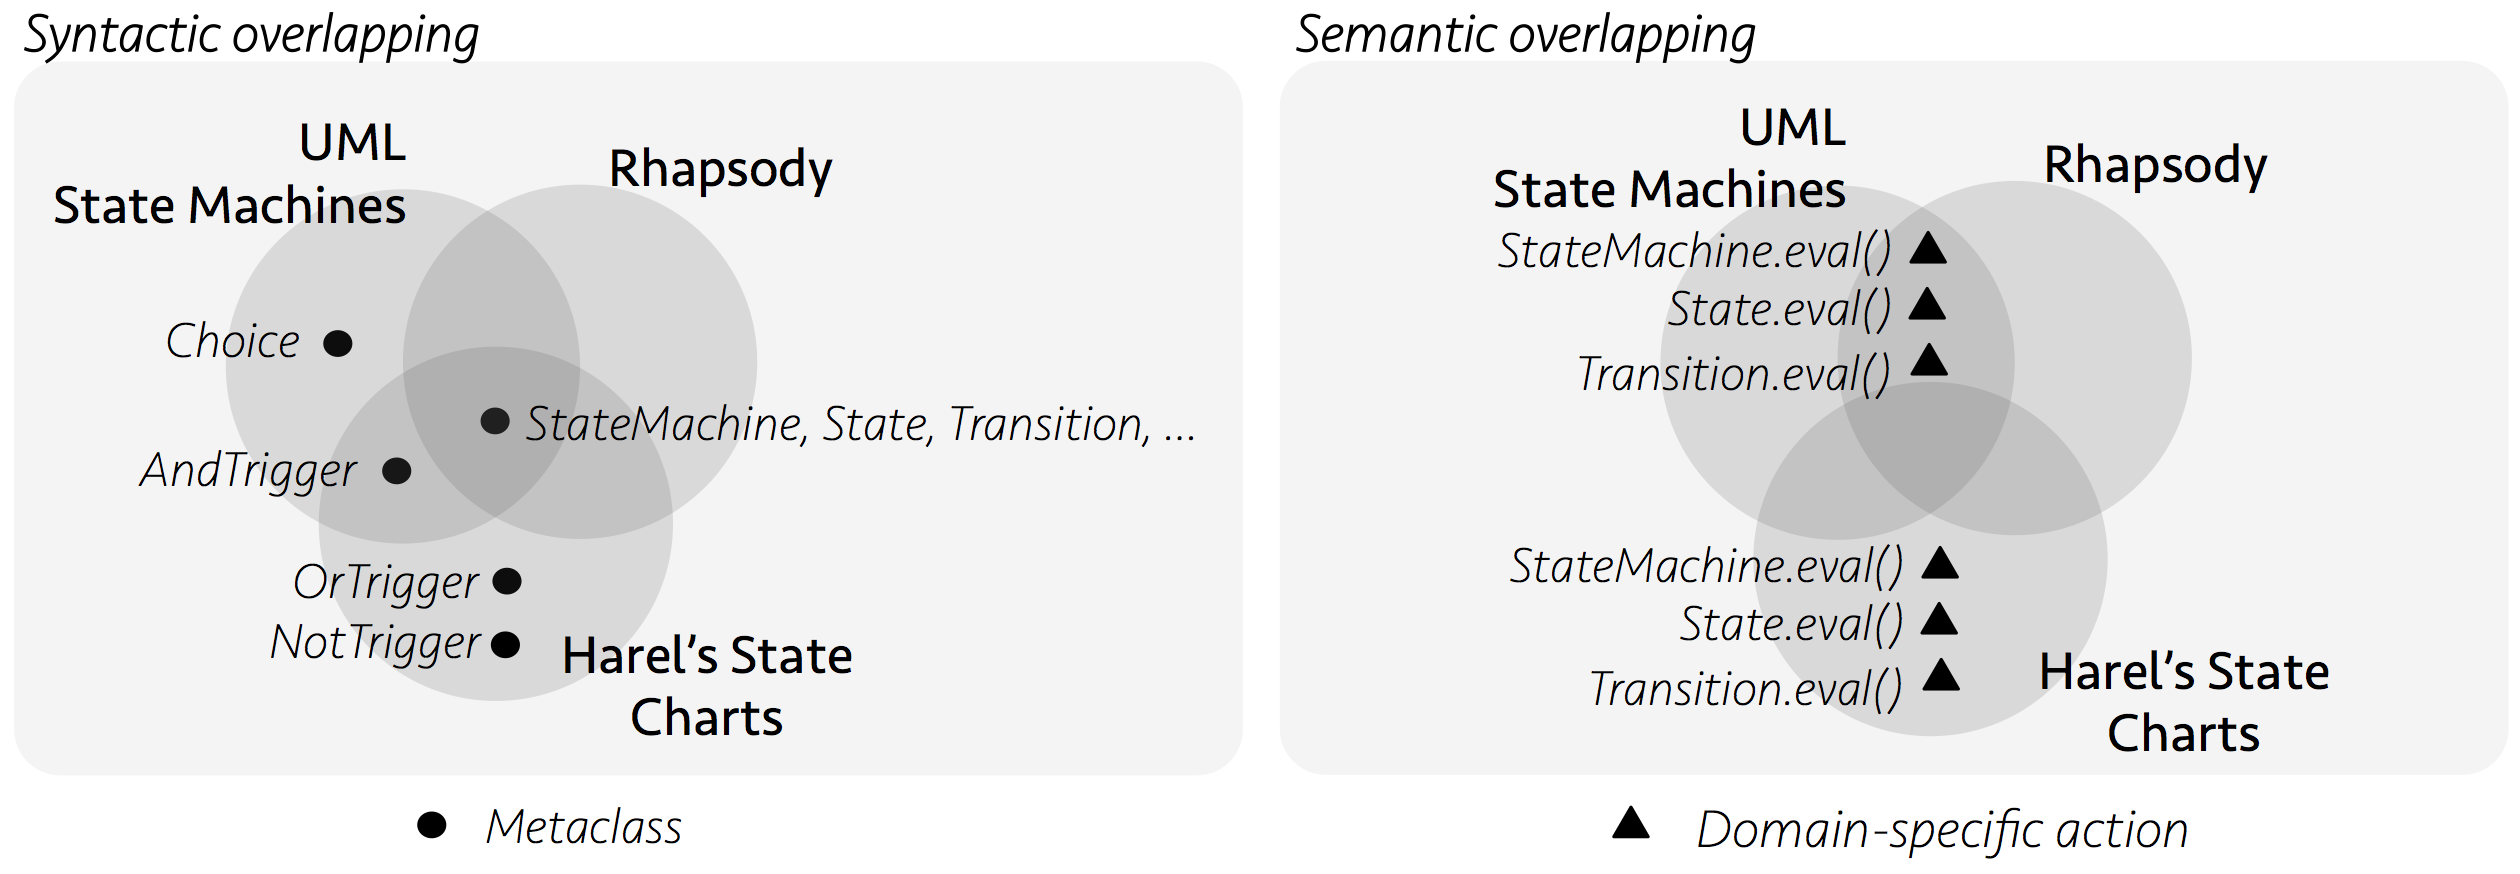
\includegraphics[width=1\linewidth]{images/fig-overlapping.png}
\caption{Syntactic and semantic overlapping in a set of DSLs}
\label{fig:shape}
\end{figure}

\vspace{2mm}
\textit{\textbf{Principle 3:} Breaking down overlapping produces reusable modules.} According to principle 2, overlapping between two DSLs implies the existence of repeated metaclasses and/or domain specific actions (i.e., specification clones). Those repeated elements can be specified once and reused in the two DSLs \cite[p. 60-61]{Voelter:2013b}. Hence, reusable language modules can be obtained by breaking down the overlapping existing among DSL specifications as illustrated in Figure \ref{fig:cutting}; each different intersection is encapsulated in a different language module. 

\begin{figure}
\centering
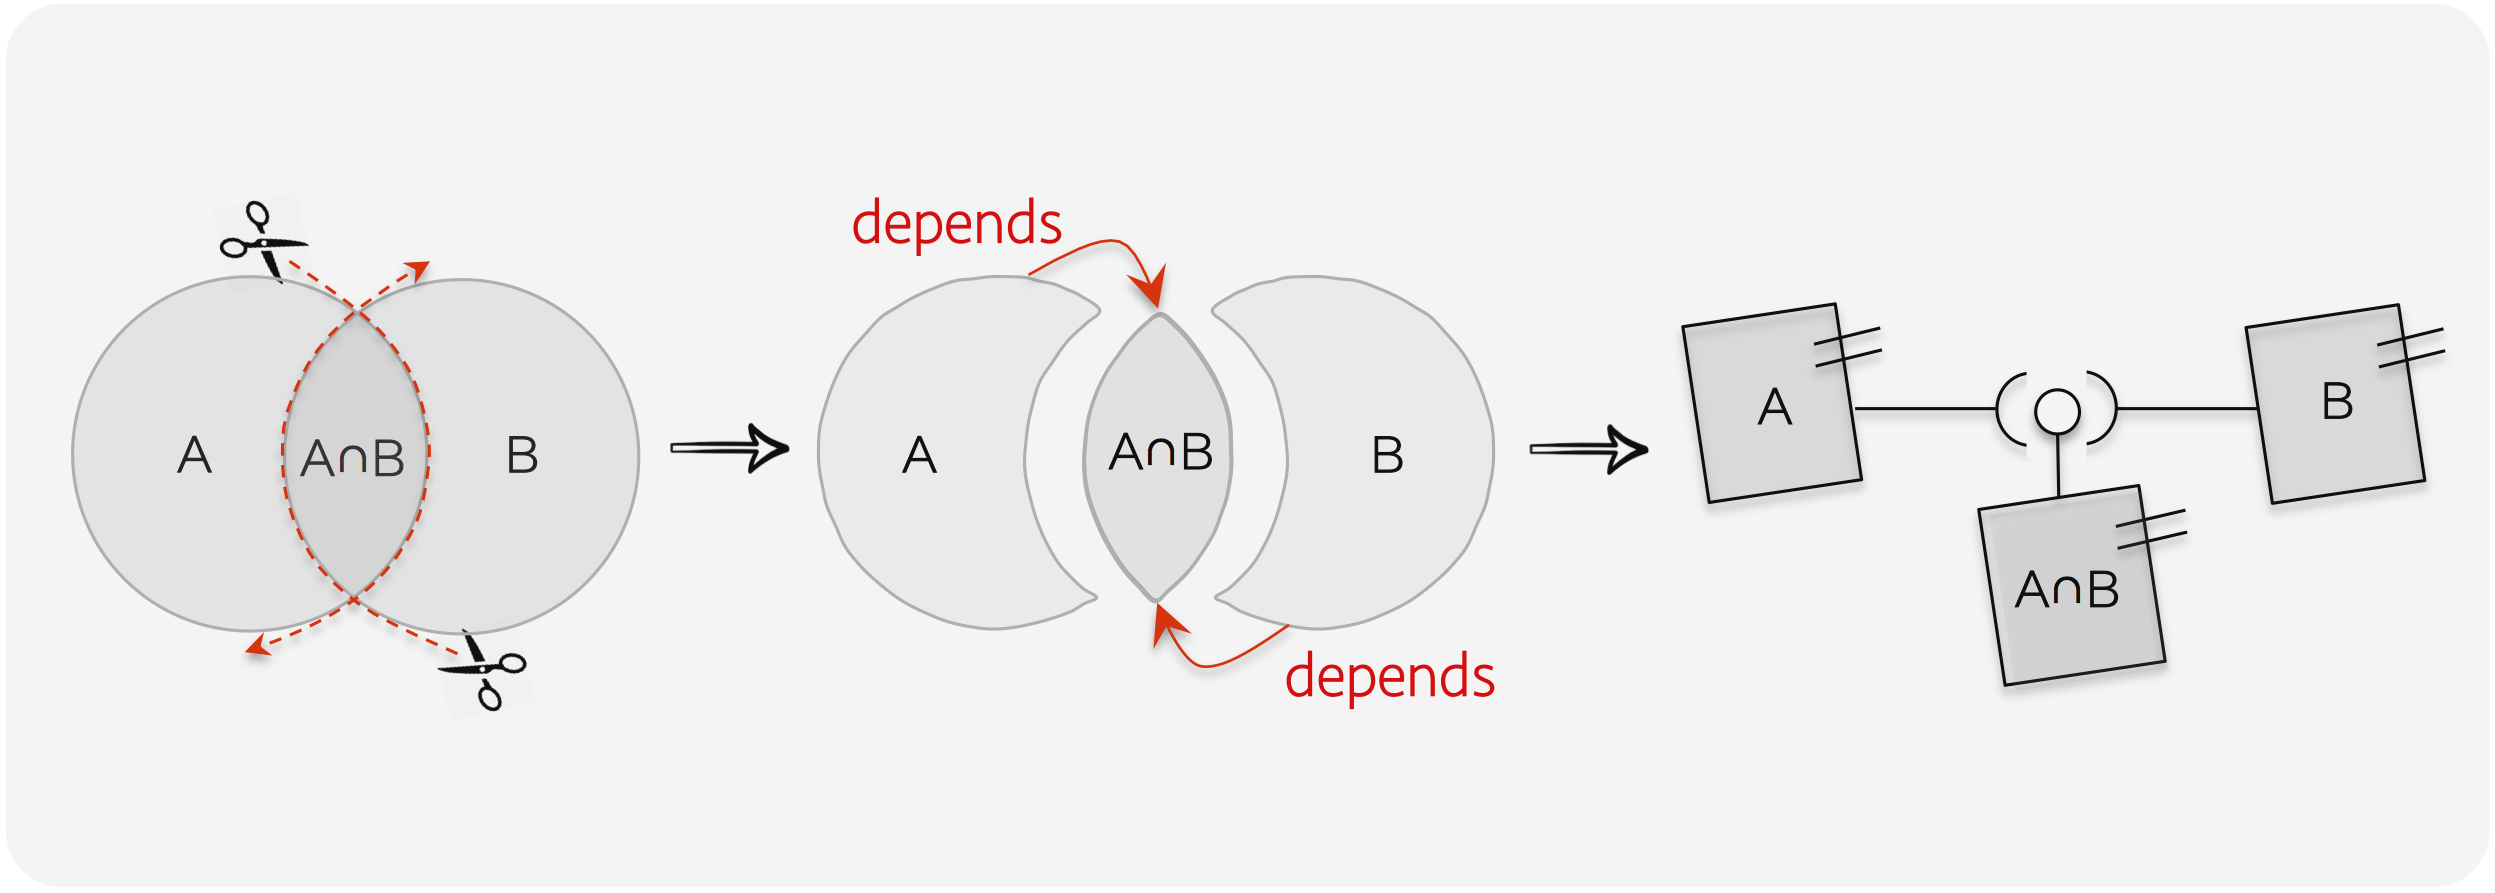
\includegraphics[width=0.97\linewidth]{images/fig-breaking-overlapping.png}
\caption{Breaking down overlapping to obtain language modules}
\label{fig:cutting}
\end{figure}

\vspace{2mm}
\textit{\textbf{Principle 4:} Abstract syntax first, semantics afterwards.} Since the abstract syntax of a DSL specifies its structure in terms of metaclasses and relationships among them, the domain-specific actions add executability to the metaclasses. Hence, the abstract syntax is the backbone of the DSL specification, and so, the process of breaking down overlapping should be performed for the abstract syntax first. Afterwards, we can do the proper for the semantics. In doing so, we need to take into consideration the phenomenon of semantic variability. That is, two cloned metaclasses might have different domain-specific actions. That occurs when two DSLs share some syntax specification but differ in their semantics.

\vspace{2mm}
\textit{\textbf{Principle 5:} Breaking down a metamodel is a graph partitioning problem.} The metamodel that specifies the abstract syntax of a DSL can be viewed as a directed graph $G$. $$G=<V,A>$$ where:

\begin{itemize}
\item \textbf{V}: is the set of vertices each of which represents a metaclass.
\item \textbf{A}: is the set of arcs each of which represents a relationships between two meta-classes (i.e., references, containments, and inheritances).
\end{itemize}

This observation is quite useful at the moment of breaking down a metamodel to satisfy the principle 4. Breaking down a metamodel can be viewed as a graph partitioning problem where the result is a finite set of subgraphs. Each subgraph represents the metamodel of a reusable language module.

\vspace{2mm}
\textbf{\textit{The 5 principles in action.}} The reverse-engineering strategy to produce a catalog of reusable modules is illustrated in Figure \ref{fig:breakingdown}. It is composed of two steps: identifying overlapping and breaking down.

\begin{figure*}
\centering
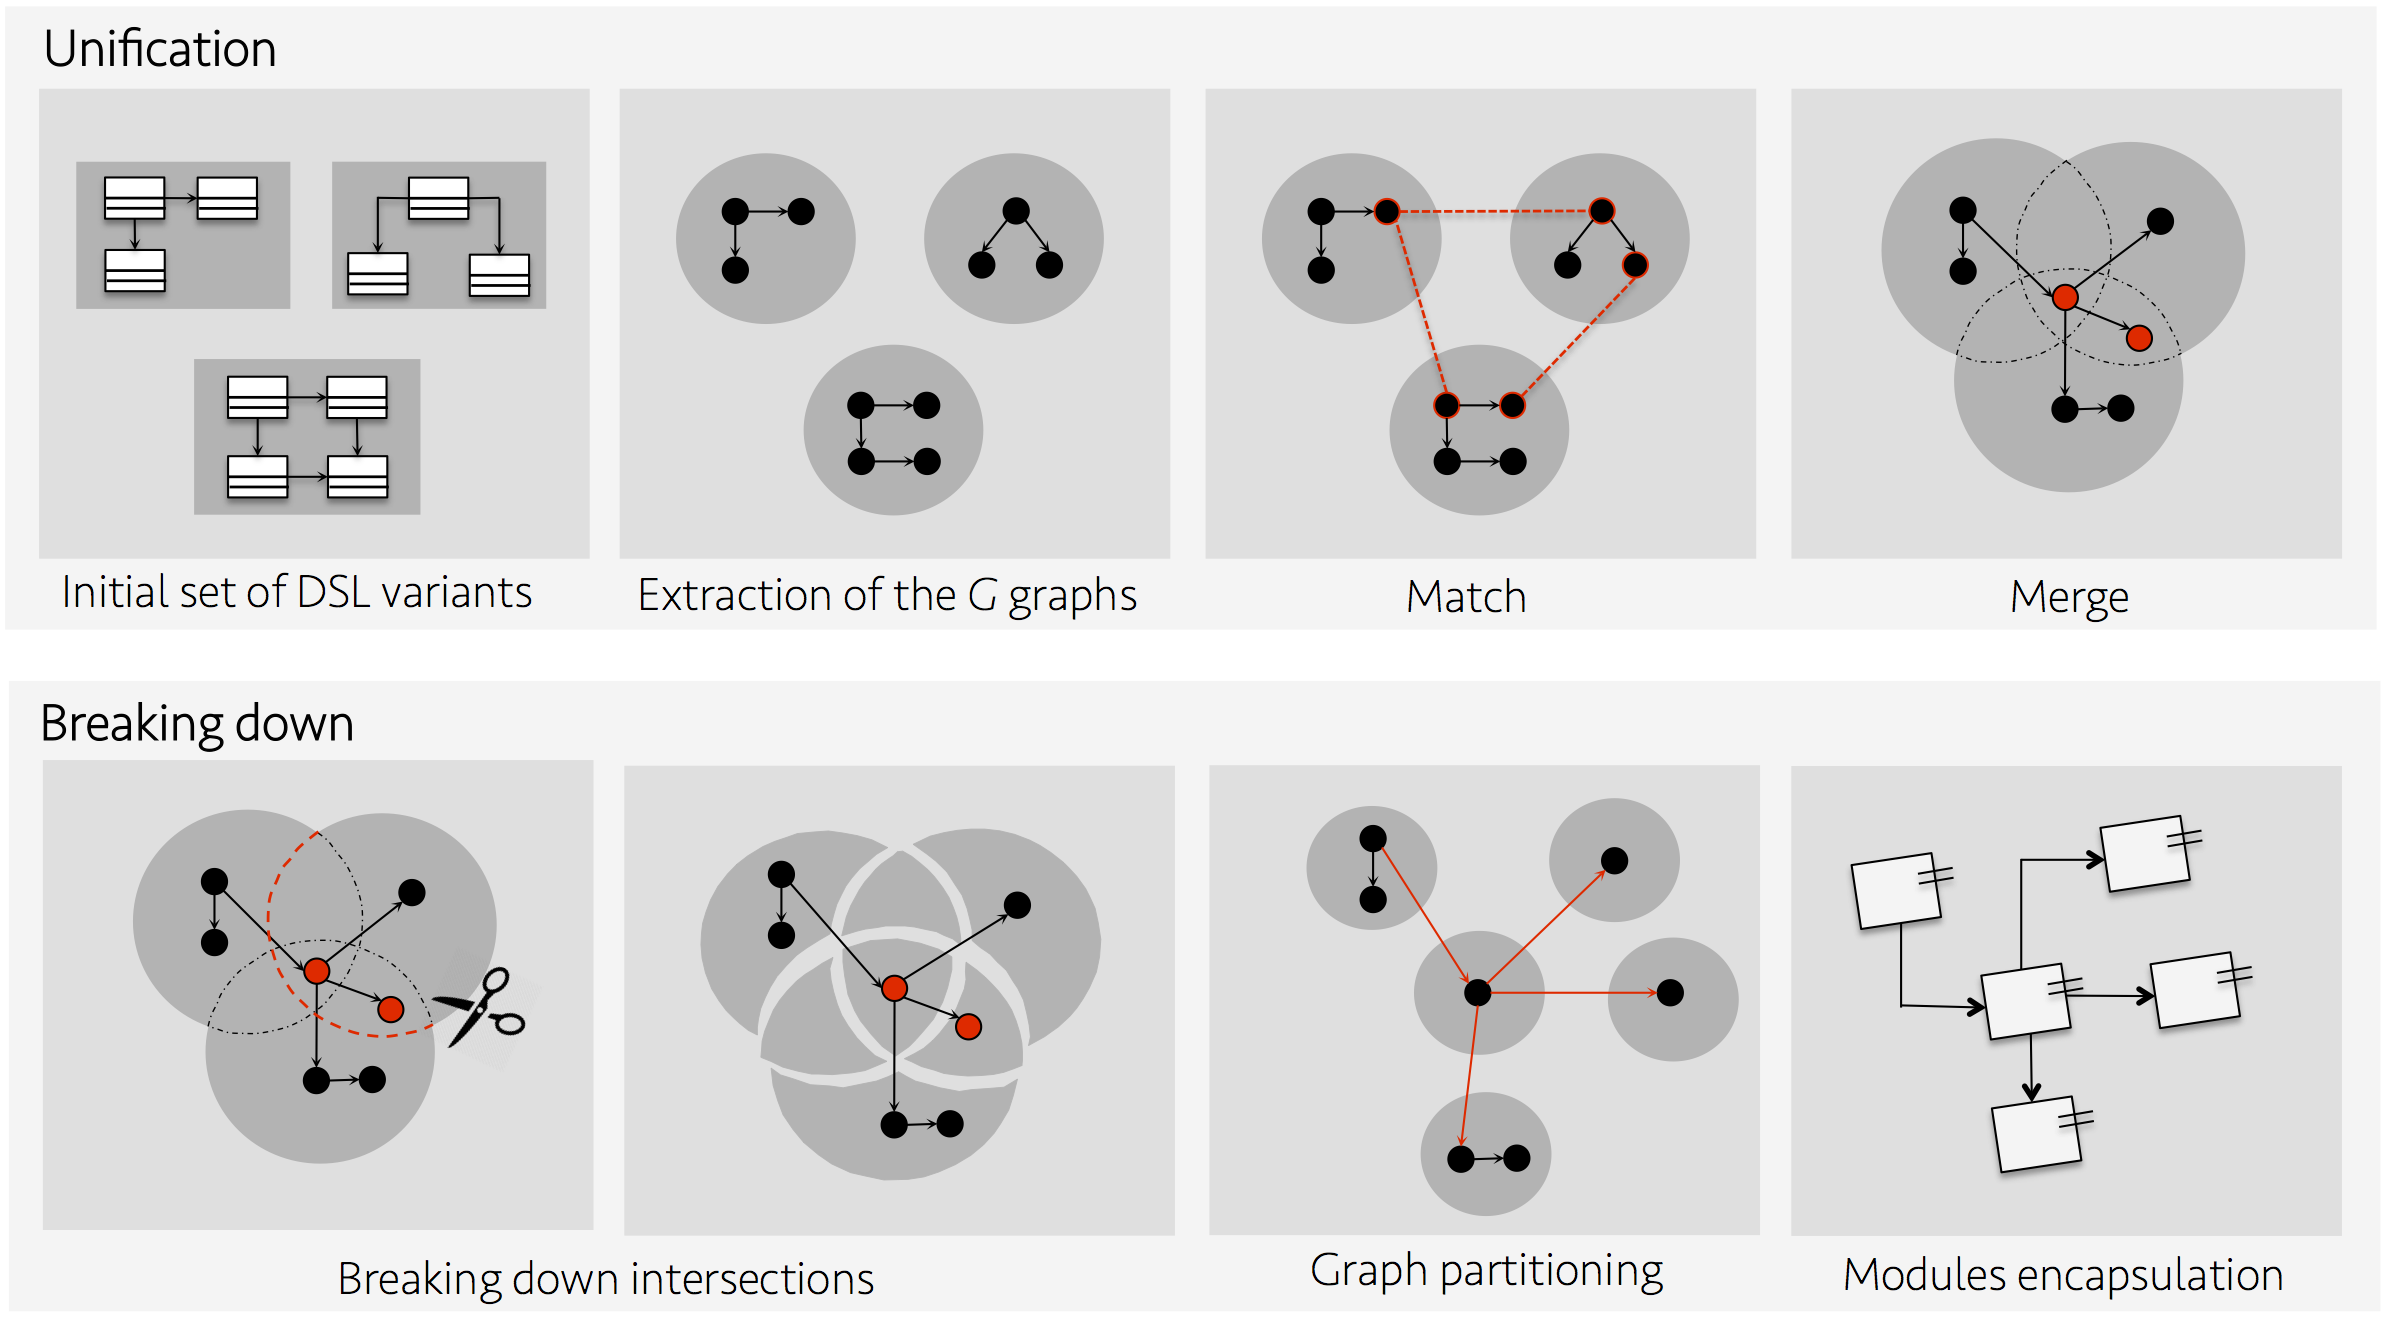
\includegraphics[width=0.8\linewidth]{images/fig-reverse-engineering-detailed}
\caption{Breaking down the input set by cutting overlapping}
\label{fig:breakingdown}
\end{figure*}

\vspace{2mm}
\textit{Identifying overlapping: \textbf{match} and \textbf{merge}.} To identify syntactic overlapping in a given set of DSLs, we start by producing a graph for each DSL according to the principle 5. Then, we identify specification clones (the matching phase) using the comparison operators defined in principle 1. After that, we have a set of graphs (one for each DSL) and a set of matching relationships among some of the vertex. At that point we can proceed to create the overlapping defined in principle 2. To this end, we merge the matched vertex as illustrated in the second square of Figure \ref{fig:breakingdown}. This merging permits to remove cloned metaclasses.

To identify semantic overlapping, we check whether the domain-specific actions of the matched metaclasses are equal as well. If so, they can be considered as clones in the semantic specification, so there is semantic overlapping. In that case, these domain-specific actions are merged. If not all the domain-specific actions associated to the matched metaclasses are the same, different clusters of domain-specific actions are created, thus establishing semantic variation points.

\vspace{2mm}
\textit{Breaking down: \textbf{cut} and \textbf{encapsulate}.} Once overlapping among the DSLs of the portfolio has been identified, we extract a set of reusable language modules. This process corresponds to break-down the graph produced in the last phase using a graph partitioning algorithm. The algorithm receives the graph(s) obtained from the merging process and returns a set of vertex clusters: one cluster for each intersection of the Venn diagram. Arcs defined between vertices in different clusters can be considered as cross-cutting dependencies between clusters. Then, we encapsulate each vertex cluster in the form of language modules. Each module contains a metamodel, a set of domain-specific actions, and a set of dependencies towards other language modules. 

Note that the dependencies between language modules can be viewed through the interfaces introduced in Section \ref{sec:meta-langauges}. Those interfaces are reverse engineered from each module. Required interfaces are generating by creating a virtual element for those elements that are required by the module but that are not part of its definition. The provided interface is generated by defining all the specification elements of the language module as public. If there are specification elements that should be hidden, then the language designer should modify the generated definition.

\subsubsection{Reverse Engineering Language Variability Models}

Once we have obtained a set of reusable language modules from a given set of DSLs, we need to represent the variability of the language product line. In other words, once we have broken down a set of existing DSLs by identifying commonalities and particularities, we need to represent those commonalities and particularities in a model that permits to configure concrete DSLs. 

To achieve such a challenge, we propose a reverse engineering algorithm to synthesize variability models from a set of reusable language modules. Our algorithm produces not only a feature model with the abstract syntax variability, but also an orthogonal variability model representing the semantic variability. An overview of the approach is presented in Fig. \ref{fig:everse-engineering-vm}, and the remainder of this section is dedicated to explain it in detail. 

\begin{figure*}
\centering
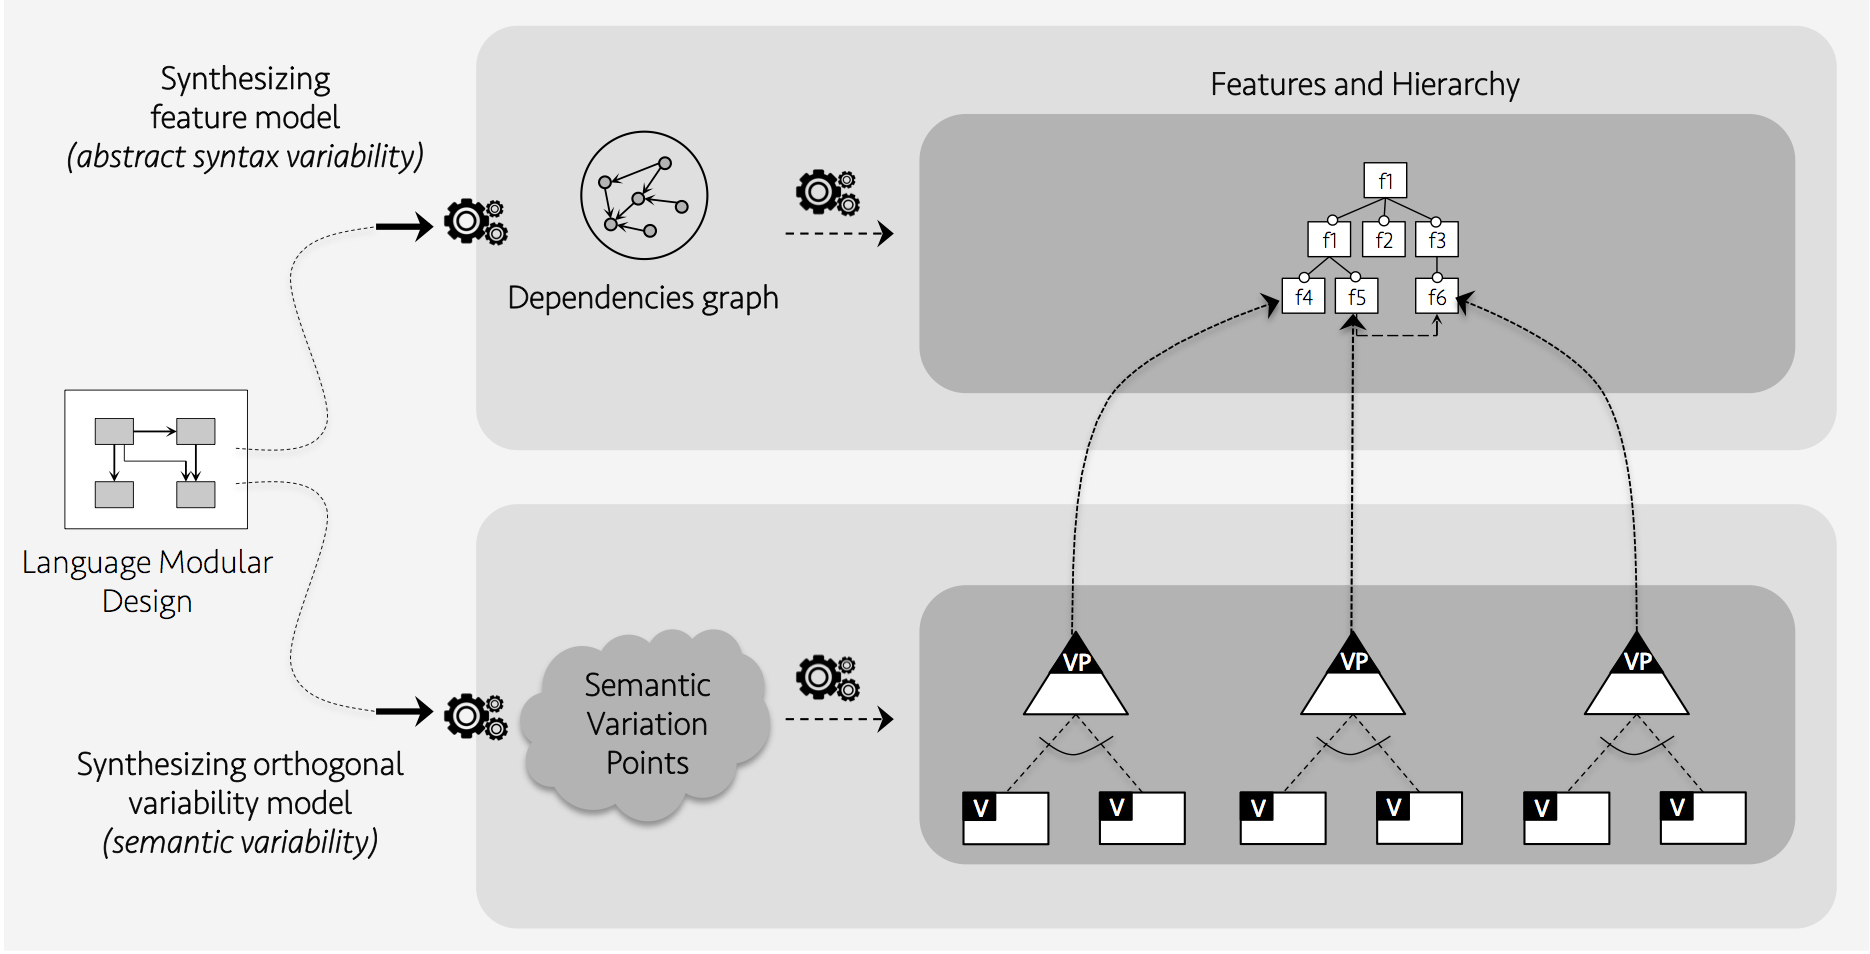
\includegraphics[width=0.8\linewidth]{images/reverse-engineering-vm.png}
\caption{Reverse-engineering variability models for language product lines}
\label{fig:everse-engineering-vm}
\end{figure*}

\vspace{2mm}
\textit{\textbf{Reverse engineering feature models representing abstract syntax variability.}} The first step to represent the variability of a language product line is to extract the feature model that represents the abstract syntax variability. To this end, we need an algorithm that receives the dependencies graph between the language modules, and produces a feature model which includes a set of features representing the given language modules as well as a set of constraints representing the dependencies among those modules. The produced feature model must guarantee that all the valid configurations (i.e., those that respect the constraints) produce correct DSLs.

In the literature, there are several approaches for reverse engineering feature modules from dependencies graphs (consider for example the approach presented by Assun\c{c}ao et al. \cite{Assuncao:2015}, or the one presented by She et al., \cite{She:2014}). In our case, we opt for an algorithm that produces a simple feature model where each language module is represented in a concrete feature, and where the dependencies between language modules are encoded either by parent-child relationships or by the classical \textit{implies} relationship. Our algorithm was inspired from the approach presented by Vacchi et al. \cite{Vacchi:2013} which fulfills the aforementioned requirements. Besides, it has been applied for the particular case of languages variability. 

The tooling that supports our algorithms is flexible enough to permit the use of other approaches for synthesis of feature model. To this end, we provide an extension point that language designers can use to add new synthesis algorithms. In addition to the one proposed by Vacchi et al. \cite{Vacchi:2013}, we have integrated our approach with the one provided by Assun\c{c}ao et al., \cite{Assuncao:2015}.

%The pseudo-code of the algorithm is introduced below; it is composed of four steps. The first step creates an abstract feature that will be used as the root feature of the variability model. The second step finds the first-level features i.e., the children of the abstract root feature. To this end, it searches all the modules that have not dependencies towards other modules. The third step finishes the hierarchy. It starts by asking the features of the first level to the dependencies they receive. For each of them they create a child. This process is repeated while there are modules that are not included in the model. Finally, we detect these dependencies that are not captured in the hierarchy and we add it in the model in the form of implies relationships. 

\vspace{2mm}
\textit{\textbf{Reverse-engineering orthogonal variability models representing semantic variability.}} Once the feature model encoding abstract syntax variability is produced, we proceed to do the proper with the orthogonal variability model encoding semantic variability. To this end, we need to analyze the results of the process for extracting the language modules. As explained in Section \ref{sec:reverseengineeringmodules}, according to the result of the comparison of the semantics, a language module might have more than one cluster of domain specific actions. This occurs when the two DSLs share constructs that are equal in terms of the abstract syntax, but differ in their semantics. Since this is the definition of semantic variation point, we materialize those clusters in semantic variation points of an orthogonal variability model.

To do this, we scan all the language modules extracted in the first phase of the reverse engineering strategy. For each language module, we verify if it has more than one cluster of domain specific actions. If so, we create a semantic variation point where each variation references one cluster. Finally, the semantic variation point is associated with the feature that represents the language module owning the clusters. 